
%(BEGIN_QUESTION)
% Copyright 2003, Tony R. Kuphaldt, released under the Creative Commons Attribution License (v 1.0)
% This means you may do almost anything with this work of mine, so long as you give me proper credit

According to the ``Ohm's Law'' formula for a capacitor, capacitor current is proportional to the {\it time-derivative} of capacitor voltage:

$$i = C {dv \over dt}$$

Another way of saying this is to state that the capacitors {\it differentiate} voltage with respect to time, and express this {\it time-derivative} of voltage as a current.  Thus, the amount of current ``through'' a capacitor is an expression of how fast the voltage {\it changes} over time.

\vskip 10pt

Suppose we had an oscilloscope capable of directly measuring current, or at least a current-to-voltage converter that we could attach to one of the probe inputs to allow direct measurement of current on one channel.  With such an instrument set-up, we could directly plot capacitor voltage and capacitor current together on the same display:

$$\includegraphics[width=15.5cm]{i01512x01.eps}$$

For each of the following voltage waveforms (channel B), plot the corresponding capacitor current waveform (channel A) as it would appear on the oscilloscope screen:

$$\includegraphics[width=15.5cm]{i01512x02.eps}$$

$$\includegraphics[width=15.5cm]{i01512x03.eps}$$

$$\includegraphics[width=15.5cm]{i01512x04.eps}$$

Note: the amplitude of your current plots is arbitrary, since I did not give you enough information (capacitor size, etc.) to actually {\it calculate} current through the capacitor at any given time.  What I'm interested in here is the {\it shape} of each current waveform, as it compares to the {\it shape} of the voltage waveform.

\underbar{file i01512}
%(END_QUESTION)





%(BEGIN_ANSWER)

$$\includegraphics[width=15.5cm]{i01512x05.eps}$$

$$\includegraphics[width=15.5cm]{i01512x06.eps}$$

$$\includegraphics[width=15.5cm]{i01512x07.eps}$$

\vskip 10pt

Follow-up question: what electronic device could perform the function of a ``current-to-voltage converter'' so we could use an oscilloscope to measure capacitor current?  Be as specific as you can in your answer.

%(END_ANSWER)





%(BEGIN_NOTES)

Here, I ask students to relate the instantaneous rate-of-change of the voltage waveform to the instantaneous amplitude of the current waveform.  Just a conceptual exercise in derivatives.

%INDEX% Mathematics, calculus: derivative (defined in a graphical sense)

%(END_NOTES)


